%# -*- coding: utf-8-unix -*-
%%==================================================
\chapter{计算机体系结构}
\label{chap1}
\begin{itemize}[noitemsep,topsep=0pt,parsep=0pt,partopsep=0pt]
	\item ...
\end{itemize}

\section{知识点和方法论}

\subsection{知识点}

\subsubsection{CPU内存模型}
多个cpu每个cpu有自己的cache缓存, 他们通过mesi协议(缓存一致性协议)和主存进行通信\
\textbf{mesi协议}
mesi协议保证了每个缓存中使用的共享变量的副本是一致的. 他的核心思想是: 当CPU写数据时候, 如果发现操作的变量是共享变量, 即在其他CPU中可存在该变量的副本, 会发出信号通知其他CPU将该变量的缓存行设置为无效状态, 当其他CPU需要读取这个变量时候, 发现自己缓存中缓存该变量的行是无效的, 那么它就会从内存重新读取.

\begin{figure}
	\centering
	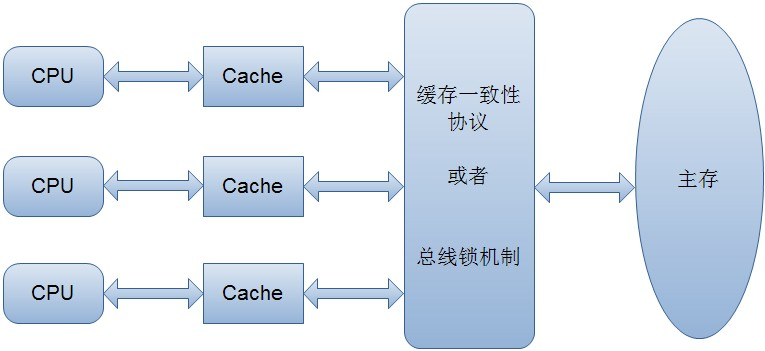
\includegraphics[width=0.7\linewidth]{figures/cpumem.jpg}
	\caption{cpumem}
	\label{fig:cpumem}
\end{figure}



\subsubsection{linux 用户态和内核态}
由于对硬件的操作涉及到驱动的调用. 这通常是不一样的. 整个操作系统为了屏蔽驱动不同的影响, 提供了一组系统调用的接口, 可以让我们利用整个机器的硬件资源, 而不用去完整理解设备的驱动逻辑.

比如我们要申请内存. 不同的内存的驱动可能是不同的, 有些内存条支持2666MHZ的频率, 但是通过系统调用可以屏蔽不同的驱动的操作方式, malloc 会调用brk()或者mmap()系统调用来分配内存.

从用户态到内核态切换可以通过三种方式:

1. 系统调用

2. 异常: 比如发生了缺页异常

3. 外设中断: 当外设完成用户的请求时候, 会向CPU发送中断信号.

\subsubsection{nginx高性能原因}
epoll 多路复用

master worker 进程模型, 平滑重启, master 重启, 然后将新的worker句柄给新的worker

协程机制 依附于线程的内存模型, 切换开销小, 与阻塞及归还执行权, 代码同步, 无需加锁

\subsubsection{bio select epoll}
bio 如果输出端满会阻塞

select  遍历, 查询效率低

epoll 模型, 变 更触发回调直接

